% !TeX document-id = {fb8a2ef5-cdaf-49da-b79d-0a8152e677cd}
% !TeX TS-program = XeLaTeX
\documentclass[a4paper,12pt]{report}

% polyglossia should go first!
\usepackage{polyglossia} % multi-language support
\setmainlanguage{russian}
\setotherlanguage{english}

\usepackage{amsmath} % math symbols, new environments and stuff
\usepackage{unicode-math} % for changing math font and unicode symbols
\usepackage[style=english]{csquotes} % fancy quoting
\usepackage{microtype} % for better font rendering
\usepackage{hyperref} % for refs and URLs
\usepackage{graphicx} % for images (and title page)
\usepackage{geometry} % for margins in title page
\usepackage{tabu} % for tabulars (and title page)
\usepackage[section]{placeins} % for float barriers
\usepackage{titlesec} % for section break hooks
\usepackage{listings} % for listings 
\usepackage{upquote} % for good-looking quotes in source code (used for custom languages)
\usepackage{xcolor} % colors!
\usepackage{enumitem} % for unboxed description labels (long ones)
\usepackage{caption}
\usepackage{multirow}
\usepackage{varwidth}
\usepackage{longtable}
\usepackage{pdfpages}

\defaultfontfeatures{Mapping=tex-text} % for converting "--" and "---"
\setmainfont{CMU Serif}
\setsansfont{CMU Sans Serif}
\setmonofont{CMU Typewriter Text}
\setmathfont{XITS Math}
\MakeOuterQuote{"} % enable auto-quotation

% new page and barrier after section, also phantom section after clearpage for
% hyperref to get right page.
% clearpage also outputs all active floats:
\newcommand{\sectionbreak}{\phantomsection}
\newcommand{\subsectionbreak}{\FloatBarrier}
\renewcommand{\thesection}{\arabic{section}} % no chapters
\numberwithin{equation}{section}
%\usetikzlibrary{shapes,arrows,trees}

\newcommand{\itemtt}[1][]{\item[\texttt{#1}:]} % tt-ed items (for protocol descriptions)

\definecolor{bluekeywords}{rgb}{0.13,0.13,1}
\definecolor{greencomments}{rgb}{0,0.5,0}
\definecolor{turqusnumbers}{rgb}{0.17,0.57,0.69}
\definecolor{redstrings}{rgb}{0.5,0,0}
\setmonofont{Consolas} %to be used with XeLaTeX or LuaLaTeX
\definecolor{bluekeywords}{rgb}{0,0,1}
\definecolor{greencomments}{rgb}{0,0.5,0}
\definecolor{redstrings}{rgb}{0.64,0.08,0.08}
\definecolor{xmlcomments}{rgb}{0.5,0.5,0.5}
\definecolor{types}{rgb}{0.17,0.57,0.68}

\lstloadlanguages{bash, python, Java}

\newcommand{\tabitem}{~~\llap{\textbullet}~~}
\newcolumntype{L}[1]{>{\raggedright\let\newline\\\arraybackslash\hspace{0pt}}m{#1}}
\newcolumntype{C}[1]{>{\centering\let\newline\\\arraybackslash\hspace{0pt}}m{#1}}
\newcolumntype{R}[1]{>{\raggedleft\let\newline\\\arraybackslash\hspace{0pt}}m{#1}}

\lstset{
  frame=none,
  xleftmargin=2pt,
  stepnumber=1,
  numbers=left,
  numbersep=5pt,
  numberstyle=\ttfamily\tiny\color[gray]{0.3},
  belowcaptionskip=\bigskipamount,
  captionpos=b,
  escapeinside={*'}{'*},
  language=python,
  tabsize=2,
  emphstyle={\bf},
  commentstyle=\it,
  stringstyle=\mdseries\rmfamily,
  showspaces=false,
  keywordstyle=\bfseries\rmfamily,
  columns=flexible,
  basicstyle=\small\sffamily,
  showstringspaces=false,
  morecomment=[l]\%,
  breaklines=true,
  showlines=true
}
\renewcommand\lstlistingname{Листинг}

\date{\today}

\makeatletter
\let\thetitle\@title
\let\theauthor\@author
\let\thedate\@date
\makeatother

\makeatletter
\AtBeginDocument{%
    \expandafter\renewcommand\expandafter\subsection\expandafter{%
        \expandafter\@fb@secFB\subsection
    }%
}
\makeatother

\begin{document}
\setcounter{page}{12}
\setcounter{section}{1}
\section{Диаграммы}
\subsection{Диаграммы прецедентов}
Комплекс при его работе предоставляет пользователю следующие варианты использования:
\begin{itemize}
  \item регистрация пользователя;
  \item авторизация пользователя;
  \item постановка задачи на исполнение;
  \item просмотр статуса задачи;
  \item отмена задачи.
\end{itemize}

Диаграмма этих и дополнительных служебных прецедентов приведена на рис.~\ref{fig:prec-common}.

\begin{figure}[b]
  \centering
  \includegraphics[width=.9\linewidth]{../diagrams/common/usecase}
  \caption{Диаграмма прецедентов всего комплекса в целом}
  \label{fig:prec-common}
\end{figure}

С учётом требований к разделению внутреннего функционала комплекса, диаграмма прецедентов на рис.~\ref{fig:prec-common}
расщепляется на набор диаграмм, соответствующих каждой из выделенных подсистем.
Соответствующие диаграммы приведены на рисунках~\ref{fig:prec-session},\ref{fig:prec-logic},\ref{fig:prec-balancer}.

\begin{figure}
  \centering
  \begin{minipage}{.49\linewidth}
    \centering
    \includegraphics[width=\linewidth]{../diagrams/session/usecase}
    \caption{Диаграмма прецедентов СУС}
    \label{fig:prec-session}
  \end{minipage}
  \hfill
  \begin{minipage}{.49\linewidth}
    \centering
    \includegraphics[width=\linewidth]{../diagrams/logic/usecase}
    \caption{Диаграмма прецедентов СУ}
    \label{fig:prec-logic}
  \end{minipage}  
\end{figure}

\begin{figure}
  \centering
  \includegraphics[width=.6\linewidth]{../diagrams/balancer/usecase}
  \caption{Диаграмма прецедентов СБН}
  \label{fig:prec-balancer}
\end{figure}

\subsection{Диаграммы действий}
Прецеденты, описанные в предыдущем пункте, отвечают определённой деятельности.
Диаграмма деятельности на рис.~\ref{fig:act-common} описывает полный процесс взаимодействия пользователя с комплексом.

С учётом требований к разделению внутреннего функционала комплекса, диаграмма деятельности на рис.~\ref{fig:act-common}
расщепляется на набор диаграмм, соответствующих определённым подсистемам из выделенных.

Диаграммы действий прецедентов подсистемы управления сессией "регистрация" и "вход в систему" приведены на рисунках~\ref{fig:act-register} и~\ref{fig:act-auth} соответственно.

Диаграммы действий прецедентов системы балансировки нагрузки "регистрация", "запрос новой задачи" и "завершение выполнения задачи" приведены на рисунках~\ref{fig:bal-register},~\ref{fig:bal-request} и~\ref{fig:bal-submit} соответственно.

Диаграммы действий прецедентов системы управления "постановка задачи" и "просмотр статсуа задачи" приведены на рисунках~\ref{fig:logic-place} и~\ref{fig:logic-view} соответственно.

\begin{figure}[h]
  \centering
  \includegraphics[width=.9\linewidth]{../diagrams/common/activity}
  \caption{Диаграмма действий прецедента "общая деятельность" для системы в целом}
  \label{fig:act-common}
\end{figure}

\begin{figure}
  \centering
  \begin{minipage}{.43\linewidth}
    \centering
    \includegraphics[width=\linewidth]{../diagrams/session/activity-register}
    \caption{Диаграмма действий прецедента "регистрация" СУС}
    \label{fig:act-register}
  \end{minipage}
  \hfill
  \begin{minipage}{.53\linewidth}
    \centering
    \includegraphics[width=\linewidth]{../diagrams/session/activity-authorize}
    \caption{Диаграмма действий прецедента "вход в систему" СУС}
    \label{fig:act-auth}
  \end{minipage}  
\end{figure}

\begin{figure}  
  \centering
  \begin{minipage}{.49\linewidth}
    \centering
    \includegraphics[width=\linewidth]{../diagrams/balancer/activity-register}
    \caption{Диаграмма действий прецедента "регистрация" СБН}
    \label{fig:bal-register}
  \end{minipage}
  \hfill
  \begin{minipage}{.49\linewidth}
    \centering
    \includegraphics[width=\linewidth]{../diagrams/balancer/activity-request}
    \caption{Диаграмма действий прецедента "запрос новой задачи" СБН}
    \label{fig:bal-request}
  \end{minipage}  
\end{figure}

\begin{figure}  
  \centering
  \begin{minipage}{.49\linewidth}
    \centering
    \includegraphics[width=\linewidth]{../diagrams/balancer/activity-submit}
    \caption{Диаграмма действий прецедента "завершение выполнения задачи" СБН}
    \label{fig:bal-submit}
  \end{minipage} 
  \hfill
  \begin{minipage}{.49\linewidth}
    \centering
    \includegraphics[width=\linewidth]{../diagrams/logic/activity-place}
    \caption{Диаграмма действий прецедента "постановка задачи" СУ}
    \label{fig:logic-place}
  \end{minipage} 
\end{figure}

\begin{figure}
  \centering
  \includegraphics[width=\linewidth]{../diagrams/logic/activity-view}
  \caption{Диаграмма действий прецедента "просмотр статсуа задачи" СУ}
  \label{fig:logic-view}
\end{figure}

\subsection{Диаграмма компонент и развёртывания}
Для того, чтобы удовлетворить требованиям по предоставлению механизма деградации функциональности,
а также для упрощения процесса разработки, комплекс должен быть разделен на отдельные слабосвязанные элементы.

Различные подсистемы комплекса имеют некую модель поведения.
Поведение подсистемы описывается её активной и пассивной частью.
Активная часть соответствует действиям, которые подсистема выполняет разово либо с некоторой периодичностью, в автоматическом режиме.
Пассивная часть соответствует API подсистемы.
Взаимосвязи между различными компонентами системы приведены на диаграмме компонентов на рис.~\ref{fig:comp-common}.
Физическое размещение компонент по отдельным узлам проиллюстрировано на диаграмме развёртывания на рис.~\ref{fig:depl-common}.

\begin{figure}[b]
  \centering
  \includegraphics[width=.7\linewidth]{../diagrams/common/component}
  \caption{Диаграмма компонент комплекса}
  \label{fig:comp-common}
\end{figure}

\begin{figure}
  \centering
  \includegraphics[width=\linewidth]{../diagrams/common/deployment}
  \caption{Диаграмма развёртывания комплекса}
  \label{fig:depl-common}
\end{figure}

\subsection{Диаграммы последовательности действий}
Диаграммы последовательности действий при выполнении прецедентов "регистрация", "запрос новой задачи" и "завершение выполнения задачи" приведены на рис.~\ref{fig:seq-reg}, \ref{fig:seq-req}~и~\ref{fig:seq-sub}.

\begin{figure}
  \centering
  \includegraphics[width=.7\linewidth]{../diagrams/frontnode/seq-register}
  \caption{Диаграмма последовательности действий прецедента "регистрация" ФВУ}
  \label{fig:seq-reg}
\end{figure}

\begin{figure}
  \centering
  \includegraphics[width=.7\linewidth]{../diagrams/frontnode/seq-request}
  \caption{Диаграмма последовательности действий прецедента "запрос новой задачи" ФВУ}
  \label{fig:seq-req}
\end{figure}

\begin{figure}
  \centering
  \includegraphics[width=.7\linewidth]{../diagrams/frontnode/seq-submit}
  \caption{Диаграмма последовательности действий прецедента "завершение выполнения задачи" ФВУ}
  \label{fig:seq-sub}
\end{figure}

\subsection{ER-диаграмма}

Связи между разными типами хранимых СХД данных предоставлены в виде ER-диаграммы на рис.~\ref{fig:db-er}.

\begin{figure}[h!]
  \centering
  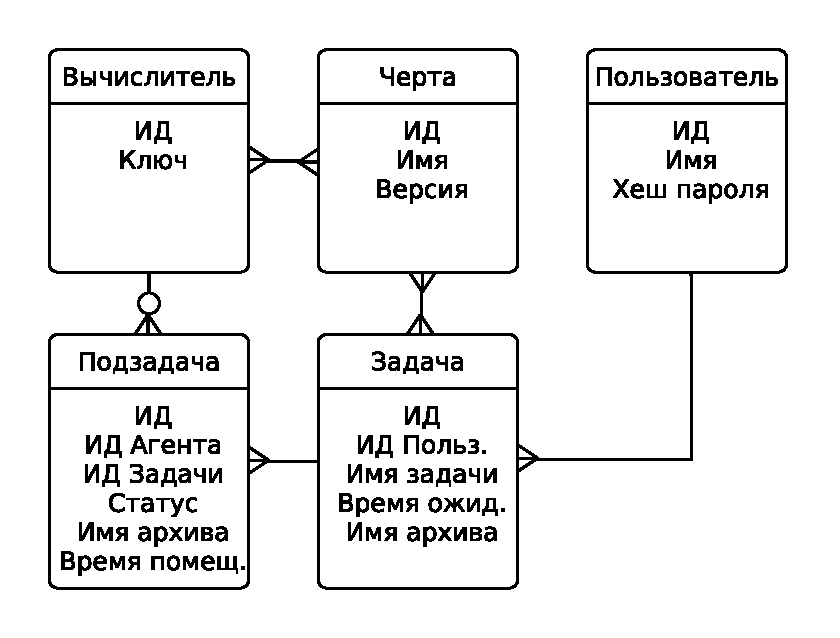
\includegraphics[width=.9\linewidth]{../diagrams/db/er}
  \caption{ER-диаграмма сущностей, хранимых в СХД}
  \label{fig:db-er}
\end{figure}

\subsection{Диаграмма состояний}
ПО вычислительного узла, обеспечивающее функционирование системы, должно удовлетворять следующим требованиям:
\begin{itemize}
  \item До подключения к серверу балансировки приложение должно предоставлять возможность формирования списка черт, характеризующих АО и ПО вычислительного узла
  \item После подключения к балансировщику (через фронтэнд вычислительных узлов), с определённой периодичностью вычислительный узел должен опрашивать комплекс на предмет наличия доступных задач
  \item По получении задачи, вычислительный узел должен с определённой периодичностью оповещать балансировщик о ходе выполнения задачи
  \item По завершении выполнения задачи, вычислительный узел должен передать балансировщику сведения о результате выполнения задачи
\end{itemize}

Диаграмма состояний ПО вычислительного узла, иллюстрирующая приведённые выше соображения, приведена на рис.~\ref{fig:node-state}.

\begin{figure}
  \centering
  \includegraphics[width=\linewidth]{../diagrams/compnode/state}
  \caption{Диаграмма состояний ВУ}
  \label{fig:node-state}
\end{figure}

\section{Тестирование}
\subsection{Модульное тестирование}
Статический класс DataMethods:


Представляет собой интерфейс бекенда данных.


Производится тестирование класса DataMethods с использованием методики тестирования -- разбиение на уровне класса на категории по функциональности. Категория объединяет в себе методы класса, выполняющие близкую по смыслу функциональность.


Методы класса можно разбить на 3 категории по функциональности:
\begin{itemize}
  \item методы получения данных;
  \item методы изменения данных;
  \item методы удаления данных. 
\end{itemize}

\begin{table}[h!]
\caption{Методы класса DataMethodsFilter}
\begin{tabu} to \textwidth {|c|X|}
\hline
Название метода & Примечания \\
\hline
\multirow{3}{*}{get\_item} & param: table [ str ] \\
                           & param: value\_json[ dict ] \\
                           & Возвращает все элементы таблицы с именем table, удовлетворяющие фильтру value\_json \\
\hline
\multirow{3}{*}{put\_item} & param: table [ str ] \\
                           & param: value\_json [ dict ] \\
                           & Изменяет все элементы таблицы с именем table, удовлетворяющие фильтру value\_json \\
\hline
\multirow{3}{*}{delete\_item} & param: table [ str ] \\
                           & param: value\_json [ dict ] \\
                           & Удаляет все элементы таблицы с именем table, удовлетворяющие фильтру value\_json \\
\hline
\end{tabu}
\end{table}

%%%
\clearpage
%%%

\begin{table}[h]
\caption{Категория 1 -- Тестирование метода получения данных}
\begin{tabu} to \textwidth {|c|X|}
\hline
Название теста & TestGetItemEmpty \\ \hline
Тестируемый метод & get\_item \\ \hline
Описание теста & Проверка получения данных из БД, пустой таблицы trait \\ \hline
Ожидаемый результат & Cловарь с пустым списком в ключе ``result'' \\ \hline
Степень важности & Фатальная \\ \hline
Результат теста & Тест пройден \\ \hline
\end{tabu}
\end{table}

%%%

\begin{table}[h]
\caption{Категория 1 -- Тестирование метода получения данных}
\begin{tabu} to \textwidth {|c|X|}
\hline
Название теста & TestGetItemGeneral \\ \hline
Тестируемый метод & get\_item \\ \hline
\multirow{4}{*}{Описание теста} & Проверка изменения данных в БД, в таблице trait, предварительно наполненной записями \\
                                & name = ``test\_name'', version = ``1.0'' \\
                                & name = ``test\_name'', version = ``2.0'', \\
                                & по фильтру \{``name'':``test\_name''\} \\
\hline
\multirow{3}{*}{Ожидаемый результат} & Словарь \{``result'':[\{``name'':``test\_name'', \\
                                & ``version'':``1.0''\}, \{``name'':``test\_name'',\} \\
                                & ``version'':``2.0''\}]\} \\
\hline
Степень важности & Фатальная \\ \hline
Результат теста & Тест пройден \\ \hline
\end{tabu}
\end{table}

%%%
\clearpage
%%%

\begin{table}[h]
\caption{Категория 2 -- Тестирование метода изменения данных}
\begin{tabu} to \textwidth {|c|X|}
\hline
Название теста & TestPutItem \\ \hline
Тестируемый метод & put\_item \\ \hline
\multirow{4}{*}{Описание теста} & Проверка изменения данных в БД, в таблице trait, предварительно наполненной записями \\
                                & name = ``test\_name'', version = ``1.0'' \\
                                & name = ``test\_name'', version = ``2.0'', \\
                                & по фильтру \{``name'':``test\_name'',``changes'': \{``version'':``3.0''\}\} \\
\hline
Ожидаемый результат & Словарь \{``count'': 2\}, отражающий наличие двух произведенных изменений в БД \\ \hline
Степень важности & Фатальная \\ \hline
Результат теста & Тест пройден \\ \hline
\end{tabu}
\end{table}

%%%

\begin{table}[h]
\caption{Категория 3 -- Тестирование метода удаления данных}
\begin{tabu} to \textwidth {|c|X|}
\hline
Название теста & TestDeleteItem \\ \hline
Тестируемый метод & delete\_item \\ \hline
\multirow{4}{*}{Описание теста} & Проверка удаления данных в БД, в таблице trait, предварительно наполненной записями \\
                                & name = ``test\_name'', version = ``1.0'' \\
                                & name = ``test\_name'', version = ``2.0'', \\
                                & по фильтру \{``name'':``test\_name''\} \\
\hline
Ожидаемый результат & Словарь \{``count'': 2\}, отражающий наличие двух произведенных удалений в БД \\ \hline
Степень важности & Фатальная \\ \hline
Результат теста & Тест пройден \\ \hline
\end{tabu}
\end{table}

\subsubsection{Вывод по результатам тестирования}
Все тесты пройдены успешно, класс готов к использованию.

\clearpage
\subsection{Системное тестирование}
Производится системное тестирования файлового сервера (стратегия чёрного ящика).
Тест покрывает все прецеденты взаимодействия с файловым сервером.

При формировании тестовых наборов использовалась методика эквивалентного разбиения для входных данных.
%При проведении тестирования сервер был запущен по адресу \url{localhost:50002}

Классы эквивалентности для входных данных:

\noindent
\begin{tabu}{|L{3cm}|L{5cm}|L{5cm}|}\hline
  Параметр & Допустимые классы эквивалентности & Недопустимые классы эквивалентности \\\hline
  Имена файлов & Строки, не содержащие символы \&,\$,/,:,*,? и другие спецсимволы & Строки, содержащие запрещённые символы \\\hline
  Адрес сервера & Строки вида 'http://address:port' & Строки, не подходящее под описание \\\hline
  Удалённый ресурс & Такие же строки, как и допустимые для имён файлов & Такие же строки, как и недопустимые для имён файлов \\\hline
  Запрос-файл & Запрос с содержимым файла в теле и с хедером 'Content-type':'multipart/form-data' & Запрос без необходимого заголовка либо испорченным телом \\\hline
\end{tabu}

\clearpage
В ходе тестирования использовался бинарный файл 'a.out', приведённый в приложении.

Тесты:

\noindent
\begin{tabu}{|L{1cm}|L{3cm}|L{2.5cm}|L{2cm}|X[l]|}\hline
  № & Описание теста & Входные данные & Ожидаемый результат & Полученный результат \\ \hline
  1 & Проверка возможности сохранения файла & Файл 'a.out' & Сообщение об успешном сохранении файла & Сообщение протокола HTTP 200 OK, пустой JSON-объект \\ \hline
  2 & Проверка доступа к существующему файлу & Запрос по адресу файла: '/static/a.out' & Содержимое файла 'a.out' & Сообщение протокола HTTP 200 OK, содержимое искомого файла \\ \hline
  3 & Проверка удаления существующего файла & Запрос на удаление файла по адресу '/static/a.out' & Сообщение об успешном удалении файла & Сообщение протокола HTTP 200 OK, пустой JSON-объект \\ \hline
  4 & Проверка удаления несуществующего файла & Запрос на удаление файла по несуществующему пути '/static/a.out' & Сообщение об ошибке & Сообщение протокола HTTP 404 NOT FOUND, JSON-объект с сообщением об ошибке \\ \hline
  5 & Проверка доступа к несуществующему файлу & Запрос по адресу несуществующего файла '/static/a.out' & Сообщение об ошибке & Сообщение протокола HTTP 404 NOT FOUND, JSON-объект с сообщением об ошибке \\\hline
\end{tabu}

\clearpage
В ходе тестирования использовались бинарные файлы 'a.out', 'b.out' и 'c.out', приведённые в приложении.

Подробное описание тестов:
\subsubsection{Тестирование надёжности и доступности серверов}
\noindent
\begin{tabu}{|L{1cm}|L{3cm}|L{2.5cm}|L{2cm}|X[l]|}\hline
  № & Описание теста & Входные данные & Ожидаемый результат & Полученный результат \\ \hline
  1 & Провести тест, в котором несколько пользователей одновременно загружают файл на сервер & Пользовательские файлы 'a.out', 'b.out' и 'c.out' & Все файлы загружены по верным адресам & Каждый из пользователей успешно загрузил файл на сервер \\\hline
  2 & Провести тест, в котором происходит разрыв соединения в ходе загрузки файла & Пользовательский файл 'a.out' & Загрузка возобновляется по восстановлении соединения & Возникла ошибка. Необходима повторная загрузка файла. \\\hline
\end{tabu}


Отчёт об обнаруженных ошибках:

\noindent
\begin{tabu}{|l|X[l]|}\hline
  \multicolumn{2}{|l|}{Сервис: файловый сервер}\\\hline
  \multicolumn{2}{|l|}{Степень важности: средняя}\\\hline
  Надёжность & Сервис некорректно отрабатывает сценарий разрыва соединения \\\hline
\end{tabu}

\subsubsection{Выводы по результатам системного тестирования}
Сервис может быть использован только в средах, где сеть можно считать достаточно надёжной. Для использования в рамках сетей где часты разрывы необходимо производить доработку сервиса.

\subsubsection{Код теста}
\lstinputlisting[language=bash]{src/queries_st.sh}

\clearpage
\subsection{Интеграционное тестирование}
Производится интеграционное тестирование подсистем работы с файлами, данными и подсистемы мониторинга. Целью тестирования явлеяется проверка
корректности регистрации подсистем на маяке, играющем ключевую роль в работе распределленной системы.

Интерфейс подсистемы мониторинга(категория -- beacon, сокращенно -- маяк):
\begin{itemize}
  \item GET /services/<service\_group>
  \item PUT /services/<service\_group>/<service\_host>:<service\_port>
  \item POST /services
\end{itemize}

Методы подсистемы работы с файлами(категория -- filesystem):
\begin{itemize}
  \item beacon\_setter
  \item beacon\_getter
\end{itemize}

Методы подсистемы работы с данными(категория -- database):
\begin{itemize}
  \item beacon\_setter
  \item beacon\_getter
\end{itemize}

\begin{table}[h]
\caption{Тестирование регистрации бекендов на не запущенном маяке}
\begin{tabu} to \textwidth {|c|X|}
\hline
Название файла & TestNoBeaconGetter.sh \\ \hline
Взаимодействующие подсистемы & database, filesystem, beacon \\ \hline
Описание теста & Подсистемы filesystem и database выполняют метод beacon\_setter при запуске \\ \hline
Начальные условия & beacon не запущен \\
Ожидаемый результат & подсистемы не могут подключиться к beacon и сообщают об этом пользователю; повторный поиск происходит регулярно, с интервалом в 10 секунд \\ \hline
Степень важности & Фатальная \\ \hline
Результат теста & Тест пройден \\ \hline
\end{tabu}
\end{table}

%%%
\clearpage
%%%

\begin{table}[H]
\caption{Тестирование регистрации бекендов на запущенном маяке}
\begin{tabu} to \textwidth {|c|X|}
\hline
Название файла & TestBeaconPoster.sh \\ \hline
Взаимодействующие подсистемы & database, filesystem, beacon \\ \hline
Описание теста & Подсистемы filesystem и database выполняют метод beacon\_setter при запуске \\ \hline
Начальные условия & beacon запущен \\
\multirow{4}{*}{Ожидаемый результат} & Подсистемы подключаются к маяку и выполняют POST-запрос на адрес /services/<категория бекенда>, 
                                       передавая через JSON свою адрес \\
                                     & Журнал маяка: \\
                                     & POST /services/database HTTP/1.1 200 \\
                                     & POST /services/filesystem HTTP/1.1 200 \\
\hline
Степень важности & Фатальная \\ \hline
Результат теста & Тест пройден \\ \hline
\end{tabu}
\end{table}

%%%

\begin{table}[H]
\caption{Тестирование регистрации бекендов на запущенном маяке}
\begin{tabu} to \textwidth {|c|X|}
\hline
Название файла & TestBeaconPutter.sh \\ \hline
Взаимодействующие подсистемы & database, filesystem, beacon \\ \hline
Описание теста & Подсистемы filesystem и database выполняют метод beacon\_setter повторно \\ \hline
Начальные условия & beacon запущен, подсистемы уже выполнили первичный POST запрос \\
\multirow{5}{*}{Ожидаемый результат} & Подсистемы подключаются к маяку и выполняют PUT-запрос на адрес \\
                                     & /services/<категория бекенда>/ \\
                                     &<адрес бекенда>:<порт>. \\
                                     & Пример журнала маяка: \\
                                     & PUT /services/database/localhost:5000 HTTP/1.1 200 \\
                                     & PUT /services/filesystem/localhost:5001 HTTP/1.1 200 \\
\hline
Степень важности & Фатальная \\ \hline
Результат теста & Тест пройден \\ \hline
\end{tabu}
\end{table}

%%%
\clearpage
%%%

\begin{table}[h]
\caption{Тестирование регистрации бекендов на запущенном маяке}
\begin{tabu} to \textwidth {|c|X|}
\hline
Название файла & TestBeaconGetter.sh \\ \hline
Взаимодействующие подсистемы & filesystem, beacon \\ \hline
Описание теста & Подсистема filesystem запрашивает адреса всех подсистем database у маяка \\ \hline
Начальные условия & beacon запущен, подсистемы уже выполнили первичный POST запрос \\
\multirow{2}{*}{Ожидаемый результат} & filesystem подключаются к маяку и выполняет GET-запрос(метод beacon\_getter)
                                       на адрес /services/database/. \\
                                      & Маяк отвечает все известные адреса бекендов, категории database
                                       в JSON-формате. Пример ответа -- [\{``localhost'': 5000\}] \\
\hline
Степень важности & Фатальная \\ \hline
Результат теста & Тест пройден \\ \hline
\end{tabu}
\end{table}


\subsubsection{Выводы по результатам интеграционного тестирования}


Интеграционное тестирование выявило фатальную ошибку в реализации подсистемы beacon, связанную с неверно документированным
поведением метода доступа к элементу по ссылке в словарях многократной вложенности в языке Python.


Ошибка была устранена с использованием альтернативной библиотечной реализации этого метода.

\section{Приложения}
\textbf{Содержимое файла a.out}

\textbf{Содержимое файла b.out}

\textbf{Содержимое файла c.out}

\end{document}